\begin{figure}[tbp]
\centering
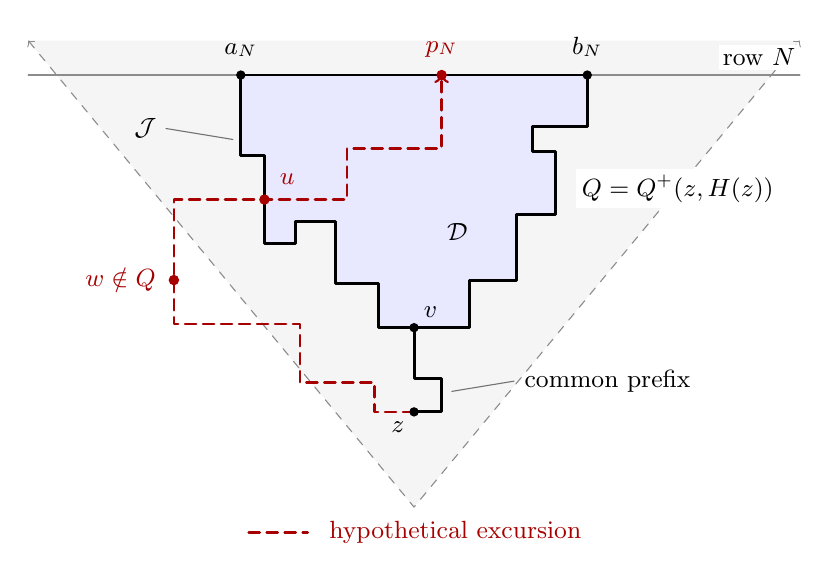
\begin{tikzpicture}[x=1cm,y=.93cm,font=\small,
  line cap=round,line join=round]
  \fill[black!4] (0,-1.3)--(-4.9,5.07)--(4.9,5.07)--cycle;
  \draw[black!45,dashed,<->] (-4.9,5.07)--(0,-1.3)--(4.9,5.07);
  \fill[blue!9!white]
    (0,1.15)--(-.45,1.15)--(-.45,1.75)--(-1,1.75)
    --(-1,2.6)--(-1.5,2.6)--(-1.5,2.3)--(-1.9,2.3)
    --(-1.9,3.5)--(-2.2,3.5)--(-2.2,4.6)
    --(2.2,4.6)--(2.2,3.9)--(1.5,3.9)--(1.5,3.55)
    --(1.8,3.55)--(1.8,2.7)--(1.3,2.7)--(1.3,1.8)
    --(.7,1.8)--(.7,1.15)--cycle;
  \draw[black!45] (-4.9,4.6)--(4.9,4.6);
  \draw[line width=.95pt] (-2.2,4.6)--(2.2,4.6);
  \node[anchor=south east,fill=white,inner sep=1.5pt]
    at (4.9,4.66) {row $N$};

  \draw[line width=1.05pt]
    (0,0)--(.35,0)--(.35,.45)--(0,.45)--(0,1.15);
  \draw[black!55] (1.27,.42)--(.48,.28);
  \node[anchor=west] at (1.28,.42) {common prefix};

  \draw[line width=1.05pt]
    (0,1.15)--(-.45,1.15)--(-.45,1.75)--(-1,1.75)
    --(-1,2.6)--(-1.5,2.6)--(-1.5,2.3)--(-1.9,2.3)
    --(-1.9,3.5)--(-2.2,3.5)--(-2.2,4.6);
  \draw[line width=1.05pt]
    (0,1.15)--(.7,1.15)--(.7,1.8)--(1.3,1.8)
    --(1.3,2.7)--(1.8,2.7)--(1.8,3.55)--(1.5,3.55)
    --(1.5,3.9)--(2.2,3.9)--(2.2,4.6);

  \draw[red!65!black,line width=.95pt,dash pattern=on 4pt off 2.5pt,->]
    (0,0)--(-.5,0)--(-.5,.4)--(-1.45,.4)--(-1.45,1.2)
    --(-3.05,1.2)--(-3.05,2.9)--(-.85,2.9)--(-.85,3.6)
    --(.35,3.6)--(.35,4.6);
  \fill (0,0) circle (1.7pt) (0,1.15) circle (1.7pt)
    (-2.2,4.6) circle (1.7pt) (2.2,4.6) circle (1.7pt);
  \fill[red!65!black] (-3.05,1.8) circle (1.9pt)
    (-1.9,2.9) circle (1.9pt) (.35,4.6) circle (1.9pt);
  \node[below left] at (0,0) {$z$};
  \node[above right] at (0,1.15) {$v$};
  \node[above=3pt] at (-2.2,4.6) {$a_N$};
  \node[above=3pt] at (2.2,4.6) {$b_N$};
  \node[above=3pt,text=red!65!black] at (.35,4.6) {$p_N$};
  \node[left=3pt,text=red!65!black] at (-3.05,1.8) {$w\notin Q$};
  \node[above right=2pt,text=red!65!black] at (-1.9,2.9) {$u$};
  \node at (.55,2.45) {$\mathcal D$};
  \node[fill=white,inner sep=2pt] at (3.35,3.05) {$Q=Q^+(z,H(z))$};
  \draw[black!55] (-3.15,3.87)--(-2.3,3.72);
  \node[left] at (-3.15,3.87) {$\mathcal J$};
  \draw[red!65!black,line width=.95pt,dash pattern=on 4pt off 2.5pt]
    (-2.1,-1.65)--(-1.35,-1.65);
  \node[anchor=west,text=red!65!black] at (-1.2,-1.65)
    {hypothetical excursion};
\end{tikzpicture}
\caption{First-arrival trapping, schematically, in $Q=Q^+(z,H(z))$.
The bounding arcs from the split $v$ to $a_N,b_N$, together with the row
segment, form $\mathcal J$ and enclose $\mathcal D\subset Q$.
The common prefix from $z$ need not lie in $\mathcal D$.
A hypothetical intermediate ray visiting $w$ outside the cone must
contact a bounding arc at $u$ before its first arrival at
$p_N\in(a_N,b_N)$, contradicting finite uniqueness. The dashed excursion
depicts this contradiction; no height monotonicity is assumed.}
\label{fig:trapping}
\end{figure}
